\begin{figure}
  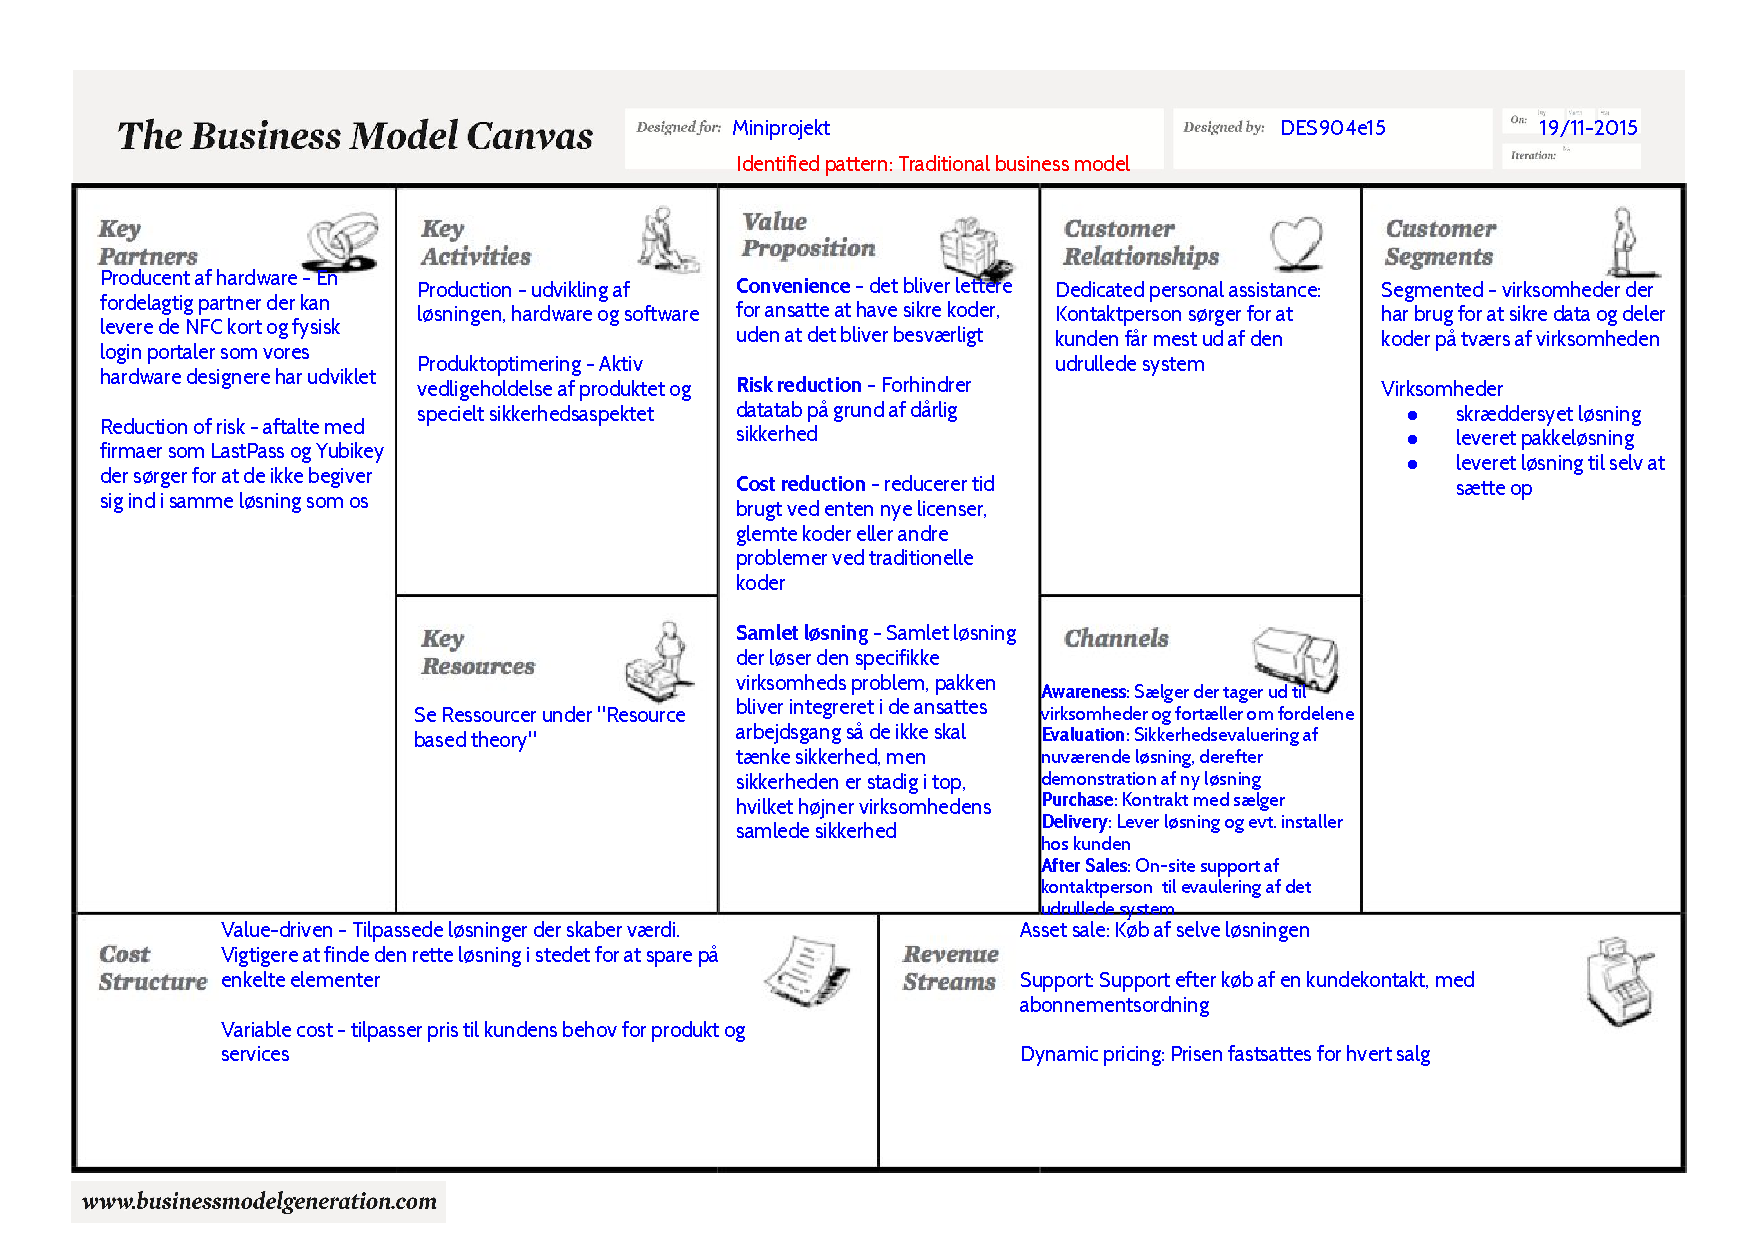
\includegraphics[angle=90, height=0.95\textheight]{graphics/BM.pdf}
  \caption{Business Model Canvas.}
  \label{bm}
\end{figure}

Nu hvor idéen er afklaret og vi har undersøgt hvordan vi vil skabe værdi kan vi begynde at designe en business model.
Vi har brugt Business Model Canvas(BMC) fra \citet{osterwalder2009business} til at komme frem til vores Business Model.
BMC kan bruges til at beskrive, designe, diskutere, udfordre, forbedre og udvikle en BM.
Det er derfor rigtig godt at bruge når man er et team med mange forskellige idéer.
Her giver BMC et rigtig godt grundlag til at få bearbejdet de forskellige idéer.


BMC består af ni elementer som sørger for at man husker alle aspekter der er vigtige når man prøver at finde på eller forbedre en BM: \textit{Customer Segments, Value Propositions, Channels, Customer Relationships, Revenue Streams, Key Resources, Key Activities, Key Partnerships, Cost Structure}.
Vores første BM kan ses på \cref{bm}.
	